
\subsection{BST}
\begin{center}
 \deff{BST} или бинарное дерево поиска.
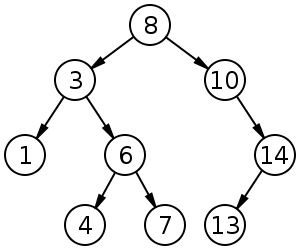
\includegraphics{assets/Binary_search_tree.png}    
\end{center}

Выполнен \textbf{инвариант}. Если x - вершина бинарного дерева со значением $k$, то все узлы в левом поддереве должны иметь ключи, меньшие $k$, а в правом поддереве большие $k$.

Все операции сделаны очень похожим образом, как у куч. Все работает за $O(h)$ дерева.

\subsection{AVL}



\deff{АВЛ-дерево} - сбалансированное двоичное дерево поиска, в котором поддерживается следующее свойство: для каждой его вершины высота её двух поддеревьев различается не более чем на 1. Адельский - Вельский, Ландис создали его.

Мы поддерживаем $h(x)$ --- количество вершин в поддереве, начинающегося с $x$.

$h(v) = max(h(L),h(R)) + 1 $.

\thmm{Лемма.}

В дереве высоты $h$ хотя бы $F_h$ вершин ($h$ - ое)

\begin{enumerate}
    \item[] \prooff{}

    Пусть $f(h)$ - min кол-во детей вершин в $AVL$ c высотой h

    $f(h) = f(h-1) + f(h-2) + 1$
\end{enumerate}

Теперь самое приятное. Как этот инвариант поддерживать?


\begin{center}
   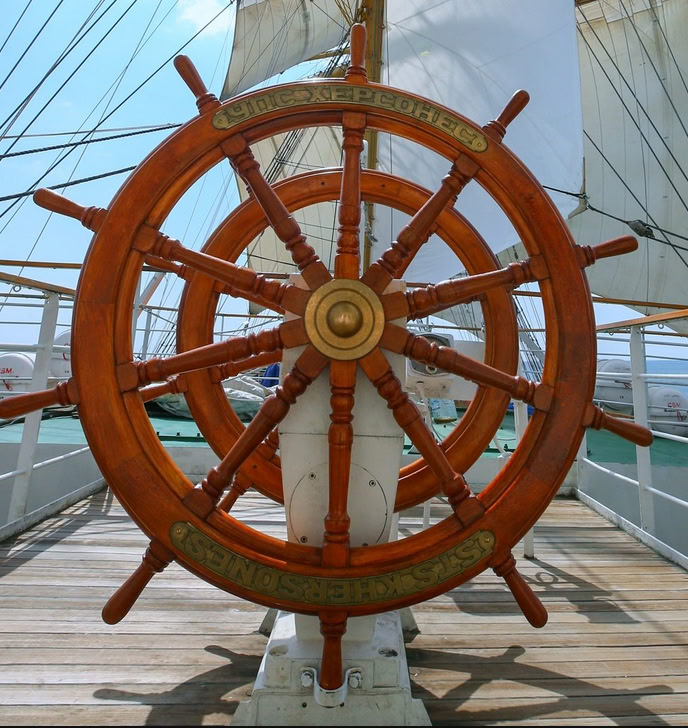
\includegraphics[width=17cm, height=17cm]{assets/wheel.jpg}
\end{center}